documentclass[tikz,border=2mm]{standalone}

\begin{document}
\begin{tikzpicture}[scale=1]
    \def\a{4}
    \draw (0,0) node[left]{\small 1} -- (\a,0) node[right]{\small 4};
    \draw (\a/3,-\a*sqrt(3)/6) -- (0,\a/2) node[left]{\small 2} -- (\a*2/3,-\a*sqrt(3)/6) node[right]{\small 3} -- cycle;
    \draw (\a*2/3,0) node[below]{\small e} -- (\a/3,0) node[below]{\small c};
    \draw (\a/2,\a/2) node{$\bullet$} node[above]{\small 1};
    \draw[ultra thick,red] (\a*2/3,\a/2) node[above]{\small 1} -- (0,\a/2+0.5) node[above]{\small s=0} node[red,right]{\small $\theta_1$} -- (\a*2/3,\a/2-0.5) node[above]{\small t=2} node[red,right]{\small $\theta_3$} ;
    \node[above] at (\a*2/3,\a/2) {\small$\gamma$};
    \node[right] at (\a*2/3,\a/2+.8) {\small$\theta_2$};
    \foreach \i/\j/\l/\t in {0/\a/0/a, 1/(\a,0)/\a/b, \a/(\a/2,\a)/\a/2,c, \a/(\a*2/3,-\a*sqrt(3)/6)/\a/3,d, (\a/3,-\a*sqrt(3)/6)/(0,\a/2)/\a/e,0/(0,\a/2)/\a/1}
        \draw[line width=.5pt,blue!\t] (\i)--(\j) node[scale=.7,above]{\scriptsize$\l$};
    \end{tikzpicture}

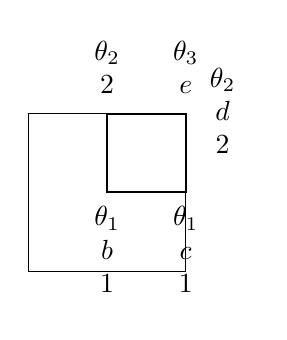
\begin{tikzpicture}[scale=1]
    \def\a{1}
    \draw (-\a,-\a) rectangle (\a,\a);
    \draw[thick] (0,\a) node[above]{$\begin{array}{c}\theta_2\\\scriptsize 2\end{array}$} -- (\a,\a) node[above]{$\begin{array}{c}\theta_3\\\scriptsize e\end{array}$} node[right]{$\begin{array}{c}\theta_2\\\scriptsize d\\2\end{array}$} -- (\a,0) node[below]{$\begin{array}{c}\theta_1\\\scriptsize c\\1\end{array}$} -- (0,0) node[below]{$\begin{array}{c}\theta_1\\\scriptsize b\\1\end{array}$} --cycle;
    \end{tikzpicture}
\end{document}